\chapter{Desenvolvimento do experimento}

Nesse capítulo é apresentado desenvolvimento do experimento, baseado nos conceitos apresentados nos capítulos anteriores. Em especial, esse capítulo mostra como as ferramentas do capítulo \ref{chap:prop} (\nameref{chap:prop}) foram utilizadas para a comparação dos algoritmos apresentados no capítulo \ref{chap:ais} (\nameref{chap:ais}).

\section{Preparação dos dados}

Os dois conjuntos de dados se encontravam em formato de texto, com os atributos separados por espaços e as instâncias separadas pelo caractere nova linha. A listagem \ref{lst:dev_data} mostra as primeiras cinco instâncias do \emph{Cr.Ger} no formato do arquivo original (a primeira coluna representa o número da linha, e não faz parte dos dados).

\vspace{0.5cm}
\begin{lstlisting}[caption=Formato original dos dados (\emph{Cr.Ger}), label=lst:dev_data]
A11 6 A34 A43 1169 A65 A75 4 A93 A101 4 A121 67 A143 A152 2 A173 1 A192 A201 1
A12 48 A32 A43 5951 A61 A73 2 A92 A101 2 A121 22 A143 A152 1 A173 1 A191 A201 2
A14 12 A34 A46 2096 A61 A74 2 A93 A101 3 A121 49 A143 A152 1 A172 2 A191 A201 1
A11 42 A32 A42 7882 A61 A74 2 A93 A103 4 A122 45 A143 A153 1 A173 2 A191 A201 1
A11 24 A33 A40 4870 A61 A73 3 A93 A101 4 A124 53 A143 A153 2 A173 2 A191 A201 2
\end{lstlisting}
\vspace{0.5cm}

A preparação dos dados para a importação no WEKA consistiu na adição de uma seção de cabeçalho e da formatação dos dados para valores separados por vírgula (seção \ref{sec:prop_arff}), e o resultado é mostrado nas listagens \ref{lst:dev_arff_ger} e \ref{lst:dev_arff_aust} (essas listagens mostram apenas as primeiras cinco instâncias na seção de dados).

\vspace{0.5cm}
\begin{lstlisting}[caption=Arquivo ARFF do \emph{Cr.Ger}, label=lst:dev_arff_ger]
@relation cr.ger

@attribute A1  {A11,A12,A13,A14}
@attribute A2  numeric
@attribute A3  {A30,A31,A32,A33,A34}
@attribute A4  {A40,A41,A42,A43,A44,A45,A46,A47,A48,A49,A410}
@attribute A5  numeric
@attribute A6  {A61,A62,A63,A64,A65}
@attribute A7  {A71,A72,A73,A74,A75}
@attribute A8  numeric
@attribute A9  {A91,A92,A93,A94,A95}
@attribute A10 {A101,A102,A103}
@attribute A11 numeric
@attribute A12 {A121,A122,A123,A124}
@attribute A13 numeric
@attribute A14 {A141,A142,A143}
@attribute A15 {A151,A152,A153}
@attribute A16 numeric
@attribute A17 {A171,A172,A173,A174}
@attribute A18 numeric
@attribute A19 {A191,A192}
@attribute A20 {A201,A202}
@attribute A21 {1,2}

@data
A11,6,A34,A43,1169,A65,A75,4,A93,A101,4,A121,67,A143,A152,2,A173,1,A192,A201,1
A12,48,A32,A43,5951,A61,A73,2,A92,A101,2,A121,22,A143,A152,1,A173,1,A191,A201,2
A14,12,A34,A46,2096,A61,A74,2,A93,A101,3,A121,49,A143,A152,1,A172,2,A191,A201,1
A11,42,A32,A42,7882,A61,A74,2,A93,A103,4,A122,45,A143,A153,1,A173,2,A191,A201,1
A11,24,A33,A40,4870,A61,A73,3,A93,A101,4,A124,53,A143,A153,2,A173,2,A191,A201,2
\end{lstlisting}
\vspace{0.5cm}

\vspace{0.5cm}
\begin{lstlisting}[caption=Arquivo ARFF do \emph{Cr.Aust}, label=lst:dev_arff_aust]
@relation cr.aust

@attribute A1  {0,1}
@attribute A2  numeric
@attribute A3  numeric
@attribute A4  {1,2,3}
@attribute A5  {1,2,3,4,5,6,7,8,9,10,11,12,13,14}
@attribute A6  {1,2,3,4,5,6,7,8,9}
@attribute A7  numeric
@attribute A8  {1,0}
@attribute A9  {1,0}
@attribute A10 numeric
@attribute A11 {1,0}
@attribute A12 {1,2,3}
@attribute A13 numeric
@attribute A14 numeric
@attribute A15 {0,1}

@data
1,22.08,11.46,2,4,4,1.585,0,0,0,1,2,100,1213,0
0,22.67,7,2,8,4,0.165,0,0,0,0,2,160,1,0
0,29.58,1.75,1,4,4,1.25,0,0,0,1,2,280,1,0
0,21.67,11.5,1,5,3,0,1,1,11,1,2,0,1,1
1,20.17,8.17,2,6,4,1.96,1,1,14,0,2,60,159,1
\end{lstlisting}
\vspace{0.5cm}

Com os arquivos no formato ARFF, os conjuntos de dados podem ser importados no WEKA. A figura \ref{fig:dev_weka_arff} mostra o conjunto de dados \emph{Cr.Ger} quando importado. Um conjunto de dados importado pode ser utilizado para qualquer algoritmo que suporte os tipos de atributos contidos nele.

\vspace{0.5cm}
\begin{figure}[h!]
    \centering
    \caption{Conjunto de dados \emph{Cr.Ger importado no WEKA}}
    \label{fig:dev_weka_arff}
    \vspace{0.5cm}
    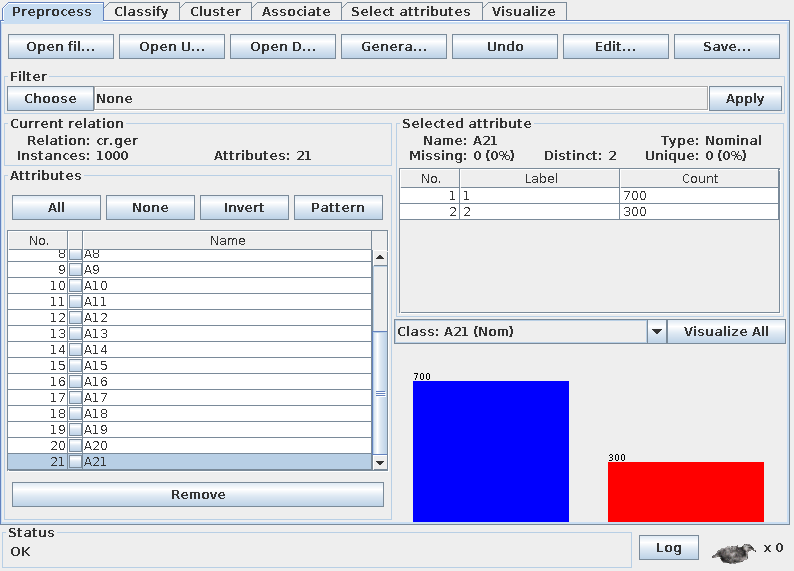
\includegraphics[width=0.75\textwidth]{img/cr_ger.png}
    \vspace{0.5cm}
\end{figure}
\vspace{0.5cm}

\section{Utilizando o WEKA}

O WEKA apresenta duas interfaces principais: linha de comando (\emph{command-line interface}, CLI\nomenclature{CLI}{Command-line Interface}) e gráfica (\emph{graphical user interface}, GUI\nomenclature{GUI}{Graphical User Interface}). A interface gráfica é mais apropriada para exploração e experimentação, e para a apresentação dos dados, algoritmos e resultados. Porém, para usos mais avançados e experimentos mais complexos, a linha de comando é mais apropriada. Além da possibilidade muito maior de automação de tarefas e exposição de opções avançadas que não estão disponíveis na interface gráfica, essa interface consume menos recursos.

Nesse trabalho foi utilizada a interface por linha de comando, já que a repetição dos testes para cada algoritmo é muito mais fácil do que se fosse utilizada a interface gráfica. Os exemplos de execução são apresentados conforme devem ser digitados em uma interface de linha de comando, em um emulador de terminal, utilizando um \emph{shell} como \emph{sh} ou \emph{bash}.

\subsection{Filtros}

No WEKA, um filtro é um objeto que recebe um conjunto de dados como entrada e produz um conjunto de dados modificado. Esse é um processo comum da Mineração de Dados, chamado de pré-processamento dos dados: adicionar, remover ou alterar atributos, etc.

Um filtro comum, que é utilizado nesse trabalho, é o de criação de partições para o \emph{cross-validation}. Para esse filtro, são passados três argumentos. O argumento \emph{c} indica qual dos atributos é o atributo correspondente à classe, e é representado por um índice, iniciado em 1, conforme a declaração na seção de atributos do arquivo de dados (caso o padrão do WEKA seja usado, ou seja, o atributo de classe seja o último da listagem, pode ser utilizado o valor ``\emph{last}'' como argumento). O argumento \emph{N} indica o número de partições, e o argumento \emph{F} indica a partição selecionada.

Além desses, o argumento \emph{V} pode ser utilizado para gerar o conjunto inverso de seleções, útil para dividir o conjunto em duas partes complementares. Dessa forma, para gerar um conjunto de dados para testes e outro para treinamento, podem ser usados os seguintes comandos\footnote{Nesses exemplos, é usado o redirecionamento de entrada e saída presentes na maioria dos \emph{shells} UNIX. O caractere ``<'' seguido de um nome de arquivo indica que aquele arquivo será usado como entrada para o comando. De maneira semelhante, o caractere ``>'' seguido de um nome de arquivo indica que ele será usado como saída. O WEKA também permite que sejam utilizadas as opções \emph{i} e \emph{o}, respectivamente, para obter os mesmos resultados. No primeiro exemplo, a forma equivalente seria ``\emph{-i dataset.arff -o dataset\_test.arff}''.}:

\begin{lstlisting}[caption=Filtro para geração de partições para \emph{cross-validation}, label=lst:dev_filter]
java weka.filters.supervised.instance.StratifiedRemoveFolds -c last -N 4 -F 1 \
    < dataset.arff > dataset_test.arff
java weka.filters.supervised.instance.StratifiedRemoveFolds -c last -N 4 -F 1 -V \
    < dataset.arff > dataset_train.arff
\end{lstlisting}

\subsection{Execução de um teste}

A execução de um algoritmo é feita através da classe que implementa o algoritmo no WEKA. Diversas opções podem ser passadas na linha de comando para mudar os parâmetros do algoritmo. Existem algumas opções adicionais para especificar dados adicionais, como os arquivos de dados para treinamento e testes. Além das opções gerais, cada algoritmo pode aceitar diferentes tipo de opções específicas. Como exemplo, para gerar a saída da listagem \ref{lst:prop_weka_out}, foi utilizado o comando da listagem \ref{lst:dev_exec_classifier}.

\vspace{0.5cm}
\begin{lstlisting}[caption=Execução de um classificador, label=lst:dev_exec_classifier]
java weka.classifiers.neural.lvq.Lvq1 -t data/weather.numeric.arff -i
\end{lstlisting}
\vspace{0.5cm}

Como é possível ver, a linha de comando é reproduzida no atributo ``\emph{Scheme}'' na saída. Esse atributo pode ser consultado para executar exatamente o mesmo teste novamente, tornando a reprodução do experimento muito mais fácil. As diversas opções do atributo que não estão presentes na linha de comando são os parâmetros do algoritmo. Como não foram especificados na linha de comando, foram assumidos os valores padrão, que são mostrados na saída. As duas opções que não estão presentes na saída são a opção ``\emph{i}'', que mostra uma saída mais completa e a opção ``\emph{t}'', que indica o arquivo que será utilizado como entrada.

Para executar os algoritmos do pacote de algoritmos imunológicos, é necessário informar à maquina virtual a localização do arquivo que contém o código executável. Esse código é disponibilizado em um arquivo \emph{jar}, um tipo de arquivo específico da linguagem java que é semelhante a um arquivo compactado utilizando os programas \emph{tar} ou \emph{zip}.

Para indicar que esse arquivo deve ser utilizado, é utilizada a opção \emph{classpath} da máquina virtual. Essa opção pode ser utilizada tanto para indicar um diretório contendo os arquivos compilados (arquivos \emph{.class}) quanto um arquivo \emph{jar}. Alternativamente, o arquivo \emph{jar} pode ser descompactado e o diretório gerado utilizado. Essa opção pode ser passada na linha de comando ou como uma variável de ambiente. Para executar o algoritmo AIRS, por exemplo, é utilizado qualquer um dos comandos da listagem \ref{lst:dev_weka_airs}. A sintaxe da opção \emph{classpath} é semelhante ao \emph{path} da maioria dos sistemas operacionais, ou seja, uma lista dos caminhos e arquivos separados pelo caractere ``:'' (dois-pontos) em sistemas Unix ou ``;'' (ponto-e-vírgula) em sistemas Windows.

\vspace{0.5cm}
\begin{lstlisting}[caption=Execução de um algoritmo do pacote de algoritmos imunológicos, label=lst:dev_weka_airs]
# Opção na linha de comando.
java -classpath wekaclassalgos.jar weka.classifiers.immune.airs.AIRS1 # parâmetros
# Variável de ambiente.
CLASSPATH=wekaclassalgos.jar
java weka.classifiers.immune.airs.AIRS1 # parâmetros
\end{lstlisting}
\vspace{0.5cm}

Combinando os conceitos apresentados nessa seção, a execução de um teste para um algoritmo imunológico utilizando um dos conjuntos de dados é feita de acordo com a listagem \ref{lst:dev_weka_single}. Aqui, é usado a opção ``\emph{t}'' para especificar o conjunto de dados \emph{Cr.Ger}. Todas as outras opções são parâmetros do filtro (os valores utilizados são os valores padrão para esse algoritmo).

\vspace{0.5cm}
\begin{lstlisting}[caption=Execução de um algoritmo do pacote de algoritmos imunológicos utilizando um dos conjuntos de dados, label=lst:dev_weka_single]
# Variável de ambiente.
CLASSPATH=wekaclassalgos.jar
java weka.classifiers.immune.airs.AIRS1 \
    -S 1 -F 0.2 -C 10.0 -H 2.0 -M 0.1 -R 150.0 -V 0.9 -A -1 -B 1 -E 1 -K 3 \
    -t german.arff
\end{lstlisting}
\vspace{0.5cm}

\subsection{Execução dos testes}

Para a execução de um teste, pode ser criado um executor genérico de classificadores, com base na listagem \ref{lst:dev_weka_single}:

\vspace{0.5cm}
\begin{lstlisting}[caption=Execução genérica de um teste, label=lst:dev_weka_template]
# Variável de ambiente.
java -classpath "$classpath" \
    "$classificador" "$parametros" -t "$conjunto_de_dados" \
    > "$arquivo_resultados"
\end{lstlisting}
\vspace{0.5cm}

Dessa forma, é possível utilizar o mesmo comando para execução, variando apenas os valores das variáveis. Os valores utilizados para cada variável foram:

\begin{enumerate}[a)]
    \item \emph{classpath}: conforme explicado na sessão anterior. Esse valor não muda entre as execuções dos testes, mas é mantido como uma variável para que ele possa ser facilmente alterado caso necessário.
    \item \emph{classificador}: essa variável tem o valor do classificador utilizado no teste.
    \item \emph{parametros}: os parâmetros para o classificador. O valor dessa variável depende do classificador utilizado.
    \item \emph{conjunto\_de\_dados}: o conjunto de dados utilizado para o treinamento e testes.
    \item \emph{arquivo\_resultados}: o arquivo onde a saída da execução será gravada.
\end{enumerate}

Para facilitar a execução de todos os algoritmos, foi utilizado um \emph{script}. O propósito desse programa é ler arquivos de configuração onde são listados os conjuntos de dados utilizados e os classificadores e executar os testes usando todas as combinações de conjunto de dados e classificador. Ou seja, esse programa recebe os classificadores e conjuntos de dados, roda os testes e grava os resultados. Mais concretamente, esse programa dá valores às variáveis descritas acima, da seguinte forma:

\begin{enumerate}[a)]
    \item \emph{classpath}: o arquivo \emph{jar} do WEKA que contém a implementação dos algoritmos imunológicos (\emph{wekaclassalgos.jar}). Esse arquivo também contém os algoritmos do WEKA, então ele é a única dependência necessária para utilizar os classificadores imunológicos e os que já são incluídos no WEKA.
    \item \emph{classificador}: todos os classificadores que foram comparados:
        \begin{enumerate}[a)]
            \item weka.classifiers.immune.airs.AIRS2
            \item weka.classifiers.immune.immunos.Immunos99
            \item weka.classifiers.immune.clonalg.CLONALG
            \item weka.classifiers.functions.MultilayerPerceptron
            \item weka.classifier.functions.SMO
            \item weka.classifiers.meta.AttributeSelectedClassifier
            \item weka.classifiers.trees.J48
            \item weka.classifiers.neural.lvq.Lvq2\_1
        \end{enumerate}
    \item \emph{parametros}: os parâmetros são listados junto com cada classificador no arquivo de configuração.
    \item \emph{conjunto\_de\_dados}: o caminho para o arquivo ARFF dos dois conjuntos de dados utilizados.
    \item \emph{arquivo\_resultados}: o nome do arquivo de saída é criado dinamicamente, combinando o nome do classificador, seus parâmetros e o nome do conjunto de dados.
\end{enumerate}

O formato exato do nome do arquivo é mostrado na listagem \ref{lst:dev_output_filename}. O objetivo desse formato é organizar os arquivos de resultados em uma hierarquia simples que facilite a implementação do programa que executa os testes e não gere diretórios com muitos arquivos.

\vspace{0.5cm}
\begin{lstlisting}[caption=Formato do nome do arquivo de resultados, label=lst:dev_output_filename]
# ex: german/AIRS1/S1_F0.2_C10.0_H2.0_M0.1_R150.0_V0.9_A-1_B1_E1_K3.txt
${dataset}/${algoritmo}/${parametros}.txt
\end{lstlisting}
\vspace{0.5cm}

Exemplos dos arquivos de configuração são mostrados nas listagens \ref{lst:dev_classifiers_json} e \ref{lst:dev_datasets_json}. Esses arquivos são lidos no formato JSON (\emph{JavaScript Object Notation}), um formato muito popular em aplicações recentes por ser de fácil leitura e escrita, tanto por humanos quanto por programas.

O primeiro arquivo lista os classificadores e seus parâmetros, o segundo os conjuntos de dados. Eles são gravados em um formato que permite que sejam facilmente transformados nas opções correspondentes na linha de comando.

\vspace{0.5cm}
\begin{lstlisting}[caption=Exemplo de arquivos de configuração de classificadores, label=lst:dev_classifiers_json]
[
    {
        "classifier": "weka.classifiers.trees.J48",
        "params": {
            "C": ["0.25"],
            "M": ["2"]
        }
    }
]
\end{lstlisting}

\begin{lstlisting}[caption=Exemplo de arquivos de configuração de conjuntos de dados, label=lst:dev_datasets_json]
[
    {
        "name": "german",
        "file": "data/statlog_german/german.arff"
    }
]
\end{lstlisting}
\vspace{0.5cm}

\subsection{Seleção de parâmetros no WEKA}

Conforme descrito no capítulo \ref{chap:eval}, o desempenho de um algoritmo depende da escolha dos parâmetros utilizados. Como o processo de escolha de parâmetros é repetitivo e fácil de ser automatizado, existem métodos para escolher os parâmetros que geram o melhor valor para os parâmetros de um modelo para um conjunto de dados específico. Um desses métodos, muito utilizado por sua simplicidade e eficácia (embora não seja tão eficiente), é o \emph{grid search}.

No WEKA, existem duas implementações desse método. Ambos fazem parte de uma categoria denominada \emph{meta-classificadores}\footnote{Esses e outros meta-classificadores que o WEKA disponibiliza podem ser encontrados no pacote \emph{weka.classifiers.meta}.}, ou seja, classificadores que atuam sobre a execução de outros classificadores. Esses dois componentes são \emph{GridSearch} e \emph{CVParameterSelection}, e seu funcionamento é semelhante. O processo para utilizá-los para a escolha de parâmetros é o seguinte:

\begin{enumerate}[a)]
    \item Utilizar um dos meta-classificadores como classificador.
    \item Indicar o classificador real que será utilizado.
    \item Listar os parâmetros que serão testados.
    \item Listar a faixa de valores para os parâmetros.
    \item Indicar o conjunto de dados que será utilizado.
    \item Executar o teste.
\end{enumerate}

Com exceção dos itens \emph{a)} e \emph{d)}, o processo é semelhante ã execução de um classificador comum. De fato, o meta-classificador executará o classificador da mesma forma que o WEKA faria. No entanto, ao invés de um única execução com parâmetros fixos, esses dois meta-classificadores fazem diversos testes, utilizando todas as combinações possíveis dos valores listados no item \emph{d)} para os parâmetros.

É importante levar em consideração que, conforme discutido anteriormente, esse processo é de grande utilidade para determinar os melhores valores para os parâmetros do classificador, no entanto, uma óbvia desvantagem é o grande aumento no tempo de execução. O número de combinações possíveis cresce exponencialmente com o número de parâmetros e número de elementos na faixa de valores para esses parâmetros.

Existem formas de amenizar o efeito da explosão combinatória desses métodos. A opção mais popular aproveita o grande potencial de paralelização do processo de execução do classificador com diferentes parâmetros. Como cada execução é completamente independente das outras, e podem ser executadas em paralelo. Na prática, grandes quantidades de unidades de processamento (denominados \emph{clusters}) são utilizados, e conjuntos de combinações de valores são distribuídas para cada um. Dessa forma, é possível aproveitar ao máximo a quantidade de recursos disponíveis. Os resultados dos testes podem então ser combinados em uma única unidade para a análise final.

\subsection{Seleção de parâmetros no experimento}

Devido ao grande número de testes executados utilizando diferentes classificadores e conjuntos de dados, não foram utilizados os métodos oferecidos pelo WEKA. O teste de um meta-classificador é feito em uma só execução e apenas o resultado final é persistido. Todos os resultados intermediários são perdidos assim que o teste é finalizado. Isso faz com que execuções subsequentes de testes que cobrem as mesmas faixas de parâmetros sejam obrigados a executar novamente testes que já foram executados.

Por exemplo, supondo que sejam executados testes conforme a listagem \ref{lst:dev_dry}. Primeiramente, é executado um \emph{grid search} utilizando o algoritmo J48 e apenas o parâmetro ``C'', o limiar de confiança, é otimizado, na faixa [0.1, 0.3]. Na segunda execução, o mesmo classificador é utilizado, porém agora é otimizado também o parâmetro ``M'', o número de instâncias por folha, na faixa [2, 10]. Todos os testes da primeira execução são perdidos assim que ela é finalizada, logo eles devem ser executados novamente na segunda execução.

\vspace{0.5cm}
\begin{lstlisting}[caption=Desperdício de recursos em execuções subsequentes, label=lst:dev_dry]
java weka.classifiers.meta.CVParameterSelection \
    -W weka.classifiers.trees.J48 -P 'C 0.1 0.3 5' \
    -t german.arff
java weka.classifiers.meta.CVParameterSelection \
    -W weka.classifiers.trees.J48 -P 'C 0.1 0.3 5' -P 'M 2 10 9' \
    -t german.arff
\end{lstlisting}
\vspace{0.5cm}

Embora esse exemplo seja simples (o número de testes do primeiro exemplo é 5 e do segundo, 45), o número de testes executados cresce exponencialmente conforme o número de parâmetros testados e a faixa de valores testados aumenta. Esse fator, combinado com um tempo de execução alto para algoritmos e conjunto de dados mais complexos, fazem com que a experimentação seja muito difícil, além de um desperdício extraordinário de recursos, já que os mesmos testes (que sempre têm o mesmo resultado) são executados repetidas vezes.

Por essas razões, foi utilizado um processo diferente para a execução dos testes. Utilizando arquivos no formato da listagem \ref{lst:dev_output_filename}, os testes podem ser executados em sequência, salvando os resultados intermediários. A qualquer momento, os arquivos existentes podem ser consultados para a avaliação dos resultados.

Um efeito colateral dessa implementação é que, como o processo que executa os testes não reexecuta um teste caso o arquivo de resultados exista, a execução dos testes pode ser dividido em diversos processos e até diversas máquinas, com a coordenação feita pelo sistema de arquivos.
